\chapter{旋轉、旋量與色對稱性}

\section{作為群的旋轉}

空間旋轉是一種對稱性，可以作用於許多種類的物件，包括剛體、速度向量、向量場和量子態。普通向量是最簡單的起點，因為它的變換可以直接想像。

旋轉也可以組合。先使物體繞一個軸旋轉某個角度，再使它繞第二個軸旋轉另一個角度。最後的取向等同於繞某個第三軸旋轉某個第三角度。因此，兩個旋轉的乘積仍是一個旋轉。

這個乘積是對變換所做的運算，不是將兩個軸向量相加。第一個旋轉會改變第二個旋轉所作用的物件。若先施行\(R_1\)，再施行\(R_2\)，組合運算便寫成\(R_2R_1\)。它本身就是某個\(R_3\)，儘管求出\(R_3\)的軸和角度可能不太方便。旋轉在複合運算下封閉，這是將旋轉視為一個群，而不只是幾何運動的集合的第一個理由。

首先以幾何方式描述一個旋轉會很有用。選取沿旋轉軸的單位向量\(\hat{\boldsymbol n}\)和角度\(\theta\)，並採用右手定則。角度為\(\theta\)的左手旋轉，也可以等價地寫成角度為\(-\theta\)的右手旋轉，或寫成繞\(-\hat{\boldsymbol n}\)的右手旋轉。

\begin{figure}[htbp]
\centering
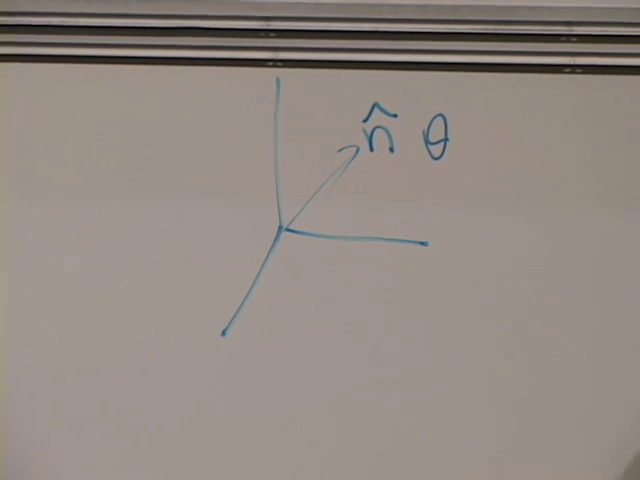
\includegraphics[width=0.58\textwidth]{lecture_03_figure_02.png}
\caption{軸\(\hat{\boldsymbol n}\)與角度\(\theta\)指定一個空間旋轉。}
\lectureframe{00:02:34}
\end{figure}

單位球面上的一個方向需要兩個參數，例如經度和緯度；繞該方向的角度則提供第三個參數。因此，旋轉構成一個三參數族。此處暫不考慮相差\(2\pi\)的角度所造成的整體等同；這裡重要的是局部參數的數目。

軸角描述有些冗餘。反轉軸並同時反轉角度，會得到相同的操作；足夠大的角度也可以對一整圈取模而化簡。這些都不影響以下事實：在恆等旋轉附近，旋轉有三個連續可變的參數。稍後會將這個局部參數數目與矩陣表示中的獨立參數數目相對應。

現在可以依序檢查群的性質：
\begin{enumerate}
\item \emph{封閉性。}連續施行兩個旋轉，結果仍是另一個旋轉。
\item \emph{恆等元。}什麼都不做就是恆等旋轉。
\item \emph{逆元。}繞\(\hat{\boldsymbol n}\)旋轉\(\theta\)，可用繞同一軸旋轉\(-\theta\)來抵消。
\item \emph{結合性。}三個連續旋轉滿足
\[
(R_1R_2)R_3=R_1(R_2R_3).
\]
\end{enumerate}

旋轉不可交換。先繞\(x\)軸旋轉，再繞\(y\)軸旋轉，通常會得到不同於反向次序的取向：
\begin{equation}
R_x(\alpha)R_y(\beta)\ne R_y(\beta)R_x(\alpha).
\end{equation}
若兩個角度都非常小，差異會是二階量，因此無窮小旋轉看起來幾乎可交換。儘管如此，整個群仍是非阿貝爾群。

不必用方程也能檢驗這種不可交換性。拿一本書或一個盒子，在其中一面標上「正面」，先繞\(x\)軸旋轉九十度，再繞\(y\)軸旋轉九十度。回到原來的取向，並反過來施行這兩個旋轉。標記的那一面最後會朝向不同方向。角度較小時，差異較難看出，但並未消失；它從兩個小角度的乘積階開始出現。

\begin{classroomqa}
\audiencequestion{這些旋轉是依序進行，而不是同時進行嗎？\lecturetimestamp{00:04:45}}
\lecturerresponse{是的。群乘法表示先做一個操作，再做另一個操作。這些連續旋轉的次序，正是可能導致不可交換的原因。}
\end{classroomqa}

這是我們遇到的第一個非阿貝爾群。最後要應用的對象不是普通物體的顏色，而是夸克的紅、綠、藍三種色態。這是一個三態的內部系統，其中有趣的變換會混合這三種顏色。普通旋轉則提供了一個熟悉的例子，說明連續群如何透過矩陣作用。

群本身是抽象的。要在物理學中使用它，就必須說明它作用於哪些物件。{表示}會為每個群元素指定一個算符或矩陣，使群元素的乘法由相應矩陣的乘法重現。同一個群可以在不同物理物件上以不同表示作用。向量、自旋一態和自旋二分之一態將作為三個例子。

\section{三維向量表示}

設普通向量的分量為
\begin{equation}
\boldsymbol V=(V_x,V_y,V_z),\qquad V_i,\quad i=1,2,3.
\end{equation}
可以固定座標軸而旋轉物理向量，也可以固定向量而旋轉座標軸。兩種約定有所不同，但無論採用哪一種，分量都會由一個\(3\times3\)矩陣混合。對每一組軸角參數\((\hat{\boldsymbol n},\theta)\)，寫成
\begin{equation}
V_i'=R_{ij}(\hat{\boldsymbol n},\theta)V_j,
\label{eq:l3-vector-rotation}
\end{equation}
其中重複指標表示求和。

重複指標\(j\)是虛指標。方程~\eqref{eq:l3-vector-rotation}明確寫出來就是
\begin{equation}
V_i'=R_{i1}V_1+R_{i2}V_2+R_{i3}V_3
\end{equation}
對每個輸出分量\(i\)都成立。自由指標\(i\)標示正在計算哪個分量；重複指標\(j\)則表示求和，可以改名而不改變方程。分清這兩種角色，就能避免長度保持論證中的大多數指標錯誤。

\begin{figure}[htbp]
\centering
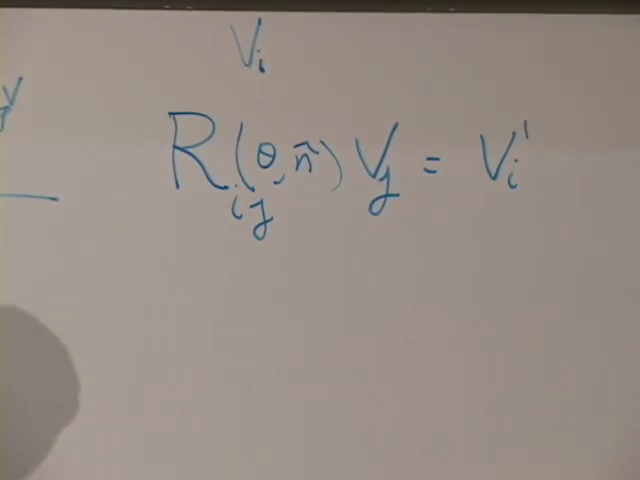
\includegraphics[width=0.68\textwidth]{lecture_03_figure_03.png}
\caption{旋轉矩陣將原向量的分量映射為旋轉後的分量。}
\lectureframe{00:07:41}
\end{figure}

真正的旋轉會保持長度。目前\(V_i\)和\(R_{ij}\)都是實數，因此
\begin{equation}
V_i'V_i'=V_iV_i
\end{equation}
對任意向量都成立。為了導出矩陣條件，以不同的虛指標寫出同一個變換：
\begin{equation}
V_i'=R_{ij}V_j,\qquad V_i'=R_{ik}V_k.
\end{equation}
相乘並對\(i\)求和，得到
\begin{align}
V_i'V_i'
 &=R_{ij}V_jR_{ik}V_k\\
 &=R_{ij}R_{ik}V_jV_k.
\end{align}
對所有\(V\)的取值，這個結果都等於\(V_jV_j\)，而這只有在
\begin{equation}
R_{ij}R_{ik}=\delta_{jk}.
\label{eq:l3-orthogonality-index}
\end{equation}
時才成立。用矩陣記號表示，
\begin{equation}
R^TR=\boldsymbol 1,
\label{eq:l3-orthogonal}
\end{equation}
因此
\begin{equation}
R^{-1}=R^T.
\end{equation}
轉置就是將行與列互換。

為什麼係數必須是\(\delta_{jk}\)？克羅內克{\proseunicodefont δ}在求和時會令\(j=k\)：
\begin{equation}
\delta_{jk}V_jV_k=V_1^2+V_2^2+V_3^2.
\end{equation}
若\(R_{ij}R_{ik}\)不等於\(\delta_{jk}\)，某個方向的長度或某個交叉項\(V_jV_k\)就會改變。由於等式必須對所有可能的向量成立，而不只是對某個特定向量成立，矩陣係數本身就必須等於單位矩陣。

方程~\eqref{eq:l3-orthogonal}是這個實矩陣表示的正交性定義條件。矩陣乘法重現了空間旋轉的乘法結構。這並非旋轉群唯一的表示，只是最容易想像的一種。

逆矩陣關係有直接的幾何意義。要抵消一個旋轉，不必另解矩陣方程，只要交換行與列即可。若\(R_1\)和\(R_2\)代表兩個旋轉，則\(R_2R_1\)代表它們依序作用的結果，而且仍是正交矩陣。因此，矩陣運算保留了幾何上已確立的封閉性、恆等元、逆元與結合性結構。

\section{自旋一與向量表示}

三維表示也會作用於量子態。自旋一粒子有三種可能的自旋投影：
\begin{equation}
m=+1,\quad 0,\quad -1.
\end{equation}
因此，它的自旋態是由三個機率振幅組成的欄向量。旋轉粒子，或改變用來定義自旋軸的磁場方向，都會透過旋轉群的三維表示來混合這三個振幅。

自旋態的數目遵循熟悉的規則\(2s+1\)。自旋零有一個態，自旋二分之一有兩個，自旋一有三個，自旋三分之二有四個。因此，態向量的維度會隨自旋而變。同一個物理旋轉作用於不同的態空間時，必須由不同大小的矩陣表示。

對自旋一粒子，選取基底
\begin{equation}
\lvert 1,+1\rangle,qquad
\lvert 1,0\rangle,qquad
\lvert 1,-1\rangle.
\end{equation}
一個態可寫成
\begin{equation}
\lvert\psi\rangle
=c_{+}\lvert1,+1\rangle+c_0\lvert1,0\rangle+c_{-}\lvert1,-1\rangle.
\end{equation}
旋轉實驗裝置不會產生第四種自旋態，而只會混合三個係數\(c_+,c_0,c_-\)。因此，相應的旋轉算符必須是\(3\times3\)矩陣。

自旋一的表示與普通空間向量遵循相同的變換方式。這就是稱自旋一粒子為\emph{向量粒子}的確切含義：它的三個自旋振幅與向量的三個分量遵循相同的旋轉定律。量子態不必想像成一支實際的箭頭；這裡說的是其分量如何混合。

這種對應並非偶然。三維向量與自旋一態承載的是旋轉群的等價三維表示。{向量粒子}一詞概括了這種變換性質，並不是說量子極化態是藏在粒子內部的一支微小剛性箭頭。

\section{離散與連續對稱性}

在討論自旋二分之一之前，先區分兩大類群會很有幫助。反射是簡單的離散例子：除了恆等操作，還有反射\(P\)；不是翻轉，就是不翻轉。相較之下，相位
\begin{equation}
e^{i\phi}
\end{equation}
會隨\(\phi\)連續變化，空間旋轉也會隨其軸和角度連續變化。這類連續群稱為\emph{李群}，名稱取自Sophus Lie；Lie讀作\emph{Lee}。本章主要關注連續對稱性，但離散對稱性也很重要。

對於包含兩個元素的反射群，
\begin{equation}
P^2=1.
\end{equation}
在\(1\)與\(P\)之間，沒有可連續調整的反射程度。相位群則不同：在\(e^{i\phi_1}\)與\(e^{i\phi_2}\)之間，還有連續無窮多個其他相位。空間旋轉也具有連續性，但與\(U(1)\)不同，旋轉是非阿貝爾的。

自旋零給出旋轉群最簡單的表示。自旋零態在所有旋轉下都不變，因此每個群元素都由一維單位矩陣表示：
\begin{equation}
D^{(0)}(R)=1.
\end{equation}
群本身仍包含無窮多個旋轉；平凡的是旋轉群在自旋零態上的表示。

群與其表示之間的區分至關重要。旋轉群作用於純量時，並不會因此縮減成只有一個元素的群；而是該群的每個元素在那個特定純量態上都由同一個數\(1\)表示。

\section{一般的自旋二分之一態}

自旋二分之一系統有兩個基底態。相對於選定的\(z\)軸，
\begin{equation}
\lvert\uparrow\rangle=
\begin{pmatrix}1\\0\end{pmatrix},
\qquad
\lvert\downarrow\rangle=
\begin{pmatrix}0\\1\end{pmatrix}.
\end{equation}
一般態是二分量旋量：
\begin{equation}
\lvert\psi\rangle=
\begin{pmatrix}\alpha_1\\\alpha_2\end{pmatrix},
\qquad
|\alpha_1|^2+|\alpha_2|^2=1.
\label{eq:l3-spinor}
\end{equation}
其分量為複數。當\((\alpha_1,\alpha_2)=(1,0)\)時，態為自旋向上；當\((0,1)\)時，態為自旋向下。一般的歸一化線性組合，描述自旋沿其他方向極化的狀態。

{向上}和{向下}只有在選定軸之後才有意義。此處選定的軸是\(z\)。不同的測量軸有不同的一對基底態；沿某一軸具有確定向上自旋的態，在另一組基底中通常會呈現為疊加態。旋轉物理自旋或參考座標軸，會相應改變其係數。

兩個複振幅包含四個實參數。歸一化條件去掉一個參數，物理上無關的整體相位再去掉一個，剩下兩個實參數。這恰好是指定球面上一個方向所需的參數數目。研究旋轉時，不必推導\((\alpha_1,\alpha_2)\)與該方向之間的明確對應關係。

整體相位可以略去，因為
\begin{equation}
\begin{pmatrix}\alpha_1\\\alpha_2\end{pmatrix}
\quad\hbox{and}\quad
e^{i\chi}
\begin{pmatrix}\alpha_1\\\alpha_2\end{pmatrix}
\end{equation}
代表同一條物理射線。歸一化固定的是總機率，而非普通歐幾里得空間中的方向。經過這兩種等同識別後，剩下的兩個參數可視為自旋極化方向的極角與方位角。

旋轉自旋後，其態變為
\begin{equation}
\alpha_i'=U_{ij}\alpha_j,
\qquad
\begin{pmatrix}\alpha_1'\\\alpha_2'\end{pmatrix}
=
\begin{pmatrix}
U_{11}&U_{12}\\
U_{21}&U_{22}
\end{pmatrix}
\begin{pmatrix}\alpha_1\\\alpha_2\end{pmatrix}.
\label{eq:l3-spinor-transform}
\end{equation}
因此，空間旋轉在旋量上有一個二維矩陣表示。這個表示具有整體的雙值性，稍後再討論；在局部範圍內，這些矩陣具備下文所需的變換性質。

變換後的二元組\((\alpha_1',\alpha_2')\)必須仍是可能的量子態。因此，關於\(U\)，首先要問的不是它明確的軸角公式，而是它必須滿足什麼條件，才能保持任意輸入旋量的歸一化。

\section{機率守恆與么正矩陣}

旋轉必須將歸一化態映射為另一個歸一化態：
\begin{equation}
\alpha_i^*\alpha_i=\alpha_i'^*\alpha_i'=1.
\end{equation}
代入方程~\eqref{eq:l3-spinor-transform}，得到
\begin{align}
\alpha_i'^*\alpha_i'
 &=(U_{ij}\alpha_j)^*(U_{ik}\alpha_k)\\
 &=\alpha_j^*U_{ij}^*U_{ik}\alpha_k.
\end{align}
因此，對應於實向量的條件是
\begin{equation}
(U^T)^*U=\boldsymbol 1.
\end{equation}
轉置後取複共軛就是厄米共軛：
\begin{equation}
U^\dagger=(U^T)^*,
\end{equation}
所以，保持歸一化的條件為
\begin{equation}
U^\dagger U=\boldsymbol 1.
\label{eq:l3-unitarity}
\end{equation}

與實向量的計算相比，唯一關鍵的差別是多了複共軛。對實向量而言，\(V_iV_i\)是長度；對旋量而言，\(\alpha_i^*\alpha_i\)是機率。為了使機率為實數且非負，必須取複共軛，因此轉置要改為厄米共軛。

方程~\eqref{eq:l3-unitarity}也立刻給出逆矩陣：
\begin{equation}
U^{-1}=U^\dagger.
\end{equation}
因此，逆旋轉也會保持相同的機率範數。和普通旋轉矩陣一樣，么正矩陣的乘積仍是么正矩陣，所以這個表示保留了群乘法結構。

\begin{figure}[htbp]
\centering
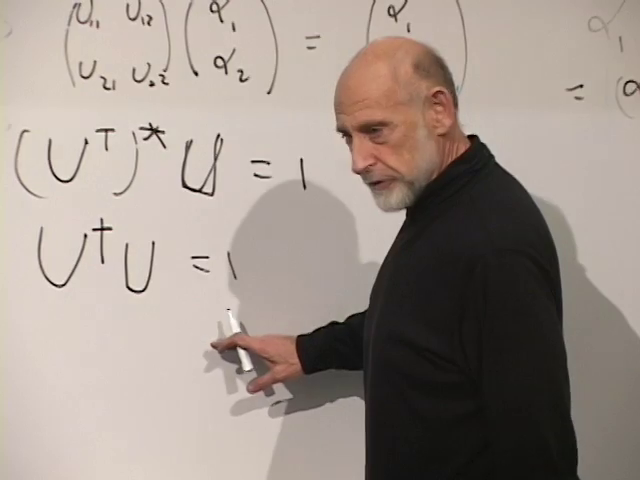
\includegraphics[width=0.62\textwidth]{lecture_03_figure_04.png}
\caption{旋量旋轉矩陣滿足\(U^\dagger U=\boldsymbol 1\)。}
\lectureframe{00:27:41}
\end{figure}

滿足方程~\eqref{eq:l3-unitarity}的矩陣稱為么正矩陣。一般的\(2\times2\)複矩陣有八個實參數。么正條件是一個\(2\times2\)矩陣方程，提供四個獨立的實約束，因此剩下四個參數。空間旋轉只有三個參數。要從整個\(U(2)\)中選出旋轉的旋量表示，還需要一個限制。

也可以將\(U\)的兩個欄視為兩個複向量，從而看出這四個約束：每個欄的範數都必須為一，這提供兩個實條件；兩欄還必須互相正交，這是一個複數條件，也就是兩個實條件。總共四個。\(U(2)\)剩下的第四個參數，最後會證明是整體行列式相位，而非新的空間旋轉。

\section{行列式為一與\texorpdfstring{\(SU(2)\)}{SU(2)}}

額外條件是
\begin{equation}
\det U=1.
\label{eq:l3-det-one}
\end{equation}
此條件與群乘法相容，因為
\begin{equation}
\det(AB)=\det A\,\det B.
\end{equation}
兩個行列式為一的么正矩陣相乘，所得矩陣的行列式仍為一；單位元的行列式也是一。這些矩陣構成一個封閉子群。

逆矩陣也屬於這個子群。若\(\det U=1\)，則
\begin{equation}
\det U^{-1}=\frac{1}{\det U}=1.
\end{equation}
因此，施加行列式為一的條件，不會移除單位元、破壞封閉性或排除逆元。這項條件一致地選出一個少一個連續參數的群。

么正性本身只推出
\begin{equation}
\det(U^\dagger U)=
(\det U)^*\det U
=|\det U|^2=1.
\end{equation}
並不能迫使\(\det U\)等於\(+1\)或\(-1\)。一般么正矩陣的行列式可以是任意相位：
\begin{equation}
\det U=e^{i\phi},
\qquad
\det U^\dagger=e^{-i\phi}.
\end{equation}
條件~\eqref{eq:l3-det-one}固定了原本自由的這個相位，並去掉一個實參數。

\begin{classroomqa}
\audiencequestion{若沒有行列式為一的條件，\(U^\dagger U=\boldsymbol 1\)是否會迫使\(\det U^\dagger\)等於\(\det U\)，或只允許\(+1\)、\(-1\)？\lecturetimestamp{00:31:21}}
\lecturerresponse{不會。兩個行列式互為複共軛；它們可以分別是\(e^{i\phi}\)和\(e^{-i\phi}\)，兩者的乘積為一。特殊么正條件則進一步將兩者都固定為一。}
\end{classroomqa}

么正的\(n\times n\)矩陣構成\(U(n)\)。當\(n=1\)時，么正矩陣就是相位\(e^{i\phi}\)，因此得到\(U(1)\)。行列式為一的子群稱為\emph{特殊么正群}：
\begin{equation}
SU(n)=\{U\in U(n):\det U=1\}.
\end{equation}
二分量旋量由\(SU(2)\)作用；這是一個三參數群。

這個記號同時表明兩項限制：\(U\)表示么正，\(S\)表示特殊，也就是行列式為一。特殊么正群會反覆出現，因為它們既保持複內積，又排除了行列式所帶有的獨立整體相位。

在局部範圍內，\(SU(2)\)具有旋轉自旋二分之一態所需的相同旋轉代數與乘法結構。在整體範圍內，則須記得先前暫緩討論的細節：\(SU(2)\)是普通旋轉群\(SO(3)\)的雙覆蓋，因此\(SU(2)\)中的兩個元素會對應到同一個空間旋轉。\editorialnote{雙覆蓋的表述，精確說明了原文提及但未展開的雙值性。}

\section{無窮小旋轉與泡利矩陣}

\begin{classroomqa}
\audiencequestion{自旋矩陣，也就是泡利矩陣，是如何出現在這個構造中的？\lecturetimestamp{00:33:16}}
\lecturerresponse{當群元素非常接近恆等元時，也就是對應到非常小角度的旋轉時，泡利矩陣便會出現。它們是這些無窮小旋轉的生成元。}
\end{classroomqa}

從
\begin{equation}
U=\boldsymbol 1+\epsilon M+O(\epsilon^2),
\label{eq:l3-small-u-anti}
\end{equation}
開始，其中\(\epsilon\)是實數且很小。於是
\begin{equation}
U^\dagger=\boldsymbol 1+\epsilon M^\dagger+O(\epsilon^2),
\end{equation}
而么正條件給出
\begin{align}
U^\dagger U
 &=\boldsymbol 1+\epsilon(M^\dagger+M)+O(\epsilon^2).
\end{align}
保留至一階可得
\begin{equation}
M^\dagger=-M.
\end{equation}
因此，方程~\eqref{eq:l3-small-u-anti}中的矩陣\(M\)是反厄米矩陣。

這裡只保留\(\epsilon\)的一次項。乘積\(\epsilon^2M^\dagger M\)是二階項，因此略去。這正是在恆等元附近運算的好處：非線性的群條件會轉化為對生成元的線性條件。

更方便的做法是提出一個\(i\)因子：
\begin{equation}
U=\boldsymbol 1+i\epsilon H+O(\epsilon^2).
\label{eq:l3-small-u-herm}
\end{equation}
複共軛會將\(i\)變為\(-i\)，因此
\begin{equation}
U^\dagger=\boldsymbol 1-i\epsilon H^\dagger+O(\epsilon^2).
\end{equation}
現在
\begin{equation}
U^\dagger U
=\boldsymbol 1+i\epsilon(H-H^\dagger)+O(\epsilon^2),
\end{equation}
一階么正條件要求
\begin{equation}
H^\dagger=H.
\end{equation}
提出\(i\)因子後，生成元便是厄米矩陣。

乘上\(i\)並未改變允許的無窮小矩陣，只改變了生成元的命名慣例。物理學通常採用厄米生成元，因為它們的本徵值為實數，且相關可觀測量（例如角動量）也是厄米的。

行列式為一的條件導出無跡條件\editorialnote{口述的行列式展開在下標處略有混淆。正確的線性項是\(A_{11}+A_{22}=\operatorname{tr}A\)；非對角項的乘積則從二階開始。}。對小的\(2\times2\)矩陣\(A\)，
\begin{equation}
\det(\boldsymbol 1+A)
=
\det
\begin{pmatrix}
1+A_{11}&A_{12}\\
A_{21}&1+A_{22}
\end{pmatrix}.
\end{equation}
展開後，
\begin{align}
\det(\boldsymbol 1+A)
 &=(1+A_{11})(1+A_{22})-A_{12}A_{21}\\
 &=1+A_{11}+A_{22}+O(A^2)\\
 &=1+\operatorname{tr}A+O(A^2).
\end{align}
將此結果用於\(A=i\epsilon H\)，得到
\begin{equation}
\det U=1+i\epsilon\,\operatorname{tr}H+O(\epsilon^2).
\end{equation}
因此，\(\det U=1\)要求
\begin{equation}
\operatorname{tr}H=0.
\end{equation}
跡條件恰好去掉與單位矩陣成正比的生成元。一般的厄米\(2\times2\)矩陣有四個實參數：兩個實數對角元素，以及一個複數非對角元素。跡條件固定其中一個實數組合，於是剩下三個參數。這與無窮小空間旋轉可選的三個旋轉軸相符。

因此，\(SU(2)\)的無窮小生成元是無跡厄米\(2\times2\)矩陣。三個泡利矩陣構成一組基底：
\begin{equation}
\begin{aligned}
\sigma_x&=
\begin{pmatrix}0&1\\1&0\end{pmatrix},
&
\sigma_y&=
\begin{pmatrix}0&-i\\i&0\end{pmatrix},
\\[0.4em]
\sigma_z&=
\begin{pmatrix}1&0\\0&-1\end{pmatrix}.
\end{aligned}
\end{equation}
每個生成元都可以寫成
\begin{equation}
H=a_x\sigma_x+a_y\sigma_y+a_z\sigma_z.
\end{equation}
繞\(x\)軸的小旋轉對應到\(\sigma_x\)；繞\(y\)軸的小旋轉對應到\(\sigma_y\)；繞其他軸旋轉則對應到相應的線性組合。在\(\hbar=1\)的單位制下，自旋算符為
\begin{equation}
S_i=\frac{\sigma_i}{2}.
\end{equation}

例如，位於\(x\)軸與\(y\)軸正中間的旋轉軸，其生成元正比於
\begin{equation}
\frac{\sigma_x+\sigma_y}{\sqrt2}.
\end{equation}
係數向量\((a_x,a_y,a_z)\)的方向決定旋轉軸；其大小與\(\epsilon\)共同決定小角度。這便是角動量對易關係中出現的自旋矩陣，與有限旋轉算符之間的關聯。特別是，
\begin{equation}
[S_x,S_y]=iS_z
\end{equation}
以及循環置換所得的關係，表達了前面從幾何上看到的不可交換性。標準的有限旋轉可由無窮小生成元取指數得到\editorialnote{指數形式的有限旋轉公式，是無窮小構造的標準延伸；原文只推導了生成元條件及其泡利矩陣基底。}，
\begin{equation}
U(\hat{\boldsymbol n},\theta)
=\exp\left(-\frac{i\theta}{2}\,
\hat{\boldsymbol n}\cdot\boldsymbol\sigma\right).
\end{equation}
\section{三態色空間}

表示的組合可以稍後再談。現在先離開空間自旋，回到夸克的色。夸克仍具有自旋二分之一，但色是另一個獨立的三態自由度：
\begin{equation}
\lvert r\rangle,\qquad
\lvert g\rangle,\qquad
\lvert b\rangle.
\end{equation}
一般的色態為
\begin{equation}
\begin{aligned}
\lvert q\rangle_{\mathrm{color}}
={}&
\alpha_r\lvert r\rangle
+\alpha_g\lvert g\rangle
+\alpha_b\lvert b\rangle,
\\
&|\alpha_r|^2+|\alpha_g|^2+|\alpha_b|^2=1.
\end{aligned}
\end{equation}
也可以寫成
\begin{equation}
q=
\begin{pmatrix}
\alpha_r\\
\alpha_g\\
\alpha_b
\end{pmatrix}.
\end{equation}
在選定的色基底下，這些係數模平方分別是測得紅、綠、藍色的機率。同樣的三分量表示法也可以將三個夸克場算符排成一個欄向量：
\begin{equation}
\psi=
\begin{pmatrix}
\psi_r\\
\psi_g\\
\psi_b
\end{pmatrix}.
\end{equation}

概念上必須區分自旋與色。自旋標籤描述態在物理空間旋轉下如何變換；色標籤描述態在不旋轉實驗室的內部對稱性下如何變換。夸克態同時帶有這兩種標籤；目前為了聚焦於色，暫不顯示自旋自由度。

將三個場算符排成一個欄向量，不只是為了方便記錄；這讓我們能用一個矩陣方程表達對稱性。變換可以將紅色場變為紅、綠、藍色場的線性組合，就如空間旋轉會將一個向量分量變為其他分量的線性組合。

可以先想像交換兩種顏色的離散變換。更大的對稱群還包含三種顏色之間的連續混合。簡單的交換矩陣可能需要乘上一個相位，才能使行列式等於一；如此一來，這種交換就會包含在特殊么正群中。

對於兩個基底態，直接交換兩者可表示為
\begin{equation}
X=
\begin{pmatrix}0&1\\1&0\end{pmatrix},
\qquad
\det X=-1.
\end{equation}
將整個矩陣乘以\(i\)後，得到
\begin{equation}
\det(iX)=i^2\det X=1.
\end{equation}
因此，只要相位選得恰當，離散交換就能成為較大連續群中的一個特定元素。

\begin{classroomqa}
\audiencequestion{只交換兩個基底態的矩陣，其行列式對\(SU(2)\)而言是否不合要求？\lecturetimestamp{00:43:46}}
\lecturerresponse{直接交換的行列式為\(-1\)。乘上適當的\(i\)因子，就能得到行列式為一的代表矩陣，因此這種交換可以包含在連續的特殊么正變換之中。}
\end{classroomqa}

\section{\texorpdfstring{\(SU(3)\)}{SU(3)}與八個色生成元}

連續的色變換為
\begin{equation}
\begin{aligned}
q'&=Uq,
&
U^\dagger U&=\boldsymbol 1,
\\
\det U&=1,
&
U&\in SU(3).
\end{aligned}
\label{eq:l3-su3-action}
\end{equation}
其數學形式與用於旋量的特殊么正構造相同，但此處\(U\)是\(3\times3\)。這不是物理空間的旋轉，而是內部色空間中的旋轉。

么正性會保持色態的歸一化：
\begin{equation}
q^\dagger q
=|\alpha_r|^2+|\alpha_g|^2+|\alpha_b|^2.
\end{equation}
行列式為一則排除了連續混合中的共同\(U(1)\)相位方向。所得矩陣可以進行簡單交換、改變相對相位，也可以形成真正的連續疊加，同時仍屬於同一個封閉群。

參數數目可以直接算出。一個\(3\times3\)複矩陣有九個複數元素，也就是十八個實參數。矩陣方程\(U^\dagger U=\boldsymbol 1\)施加九個實條件；行列式為一再去掉一個參數：
\begin{equation}
\dim SU(3)=18-9-1=8.
\end{equation}
因此，\(SU(3)\)有八個獨立的無窮小生成元。

也可以透過\(U\)的欄來理解這九個么正條件。三個複數欄向量各自都必須具有單位範數，而且每一對都必須互相正交。這些條件從原有的十八個實參數中去掉九個；行列式的相位再去掉第十個，剩下八個。這是三態情形下，\(SU(2)\)的\(8-4-1=3\)參數計數的對應情形。

八這個數字的出現，與最終得到八種膠子，是同一個事實所致。說膠子之所以不是九種，是因為行列式限制移除了一個方向，這只是一種助記說法。更精確地說，九個色－反色矩陣可分解為一個與單位矩陣成正比的色單態方向，以及八個無跡方向。這八個無跡生成元構成 QCD 膠子所承載的伴隨色結構。\editorialnote{單態加八重態的表述，是對原文刻意採用的啟發式行列式說法所作的標準精確詮釋；規範場的構造留待後續討論。}

此時，八種膠子與前述結果的關聯只是提示，還不是完整的推導。要得到規範粒子，必須將色對稱性提升為局域對稱性，並確定補償場。參數計數已經表明，在\(SU(3)\)色變換中，有八個獨立方向可使變換從單位元開始偏離。

\section{色對稱性對 QCD 的約束}

基本的對稱性敘述是：物理定律在方程式~\eqref{eq:l3-su3-action}所示的色變換下保持不變。這是量子色動力學的核心內部對稱性。色分量的混合在形式上類似於自旋向上與自旋向下振幅的混合；而那些旋量變換又與空間方向的旋轉相關，但這三種空間不可混為一談。

稱色為一種對稱性，意指改變色基底不會改變物理預測。紅、綠、藍是三個基底向量的方便稱呼，並非三種可觀測的顏料。對色分量同時施行\(SU(3)\)旋轉，必須使定律的形式保持不變。這種不變性並非可有可無的美學特徵，而是 QCD 的組織原則。

對稱性會限制拉格朗日量。在先前的\(U(1)\)例子中，對共同相位變換的不變性，限制了允許出現的項，使其包含場與其共軛場的平衡因子。在 QCD 中，每一項同樣都必須在\(SU(3)\)色變換下保持不變。這項要求會影響相互作用、守恆量，以及膠子場的形式。

假設某個候選項帶有一個未縮併的色指標。在方程式~\eqref{eq:l3-su3-action}所示的變換下，該指標會旋轉，因此此項本身無法保持不變。允許的項必須將色指標縮併成不變組合，或使用變換能補償這項變化的規範場。這就是對稱性原理的實際作用：它排除任意耦合，並規範剩餘相互作用的形式。

QCD 的完整構造還需要進一步處理：必須允許色變換隨位置改變，並由規範場補償這種局域變化。\editorialnote{將色對稱性局域化，是全域\(SU(3)\)討論在規範理論中的標準延伸；本講稿並未展開這部分。}這部分內容留待下一階段。目前，基本結構已經建立：色三重態受到具有八個生成元的三態特殊酉對稱性作用。

目前所需的群論計算已經完成。我們從能在普通空間中描繪的旋轉出發，進而討論作用於向量和旋量的矩陣，再把同樣的邏輯運用到內部色空間。下一步可以在已有數學架構的基礎上回到粒子物理，而不必讓形式體系一次承載全部物理內容。